\section{Project Implementation}
The projects goal is a way to mandate security with low false positives. The start of this project involved creating a list of checks to implement as shown in Figure~\ref{fig:fig1}.
\begin{figure}[!ht]
  \centering
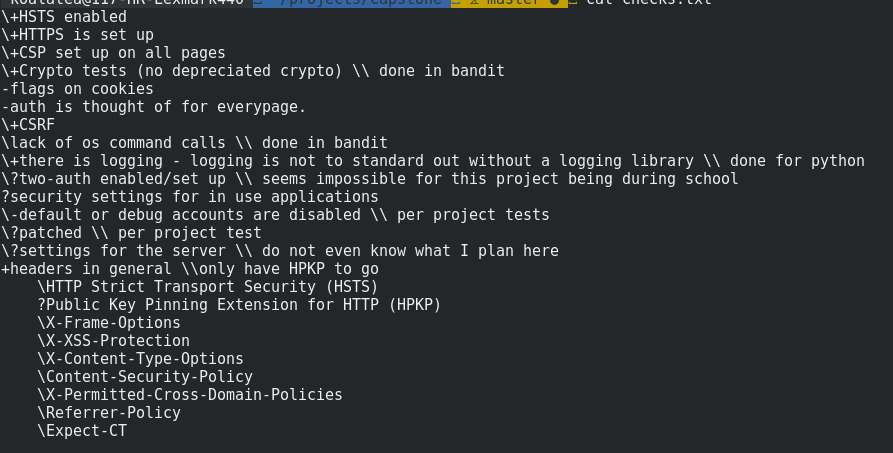
\includegraphics[width=4in]{unittestchecks}
\caption{\label{fig:fig1}}The list of checks to implement
\end{figure}
The checks were chosen for both their ease of being checked and their security relevance. Tests that could be dynamic were prioritized over those that had to be static. The notation in 
Figure~\ref{fig:fig1} checks is that a leading $\backslash$ means the test is addressed, a + means that the test has been chosen to be implmented, a - meant the test would not be implemented, and a ?
meant that their are still questions about the test. The majority of tests implemented are headers, with each one making specifc bugs harder to exploit.

The implemented tests were all of the headers tests, and the logging test. The depreciated crypto test and the os test were both found to be done for python in the bandit source code analysis tools
\cite{bandit}. The HPKP header was dropped due to it's pending removal from chrome in favor of the new Expect-CT header \cite{hpkp}. The headers are chosen because they are easy to test for
dynamically, the same rational applies to csrf and https. The only static test that is created for this project is the logging test one because it does not require context like authentication being
addressed for every web page. Figure~\ref{fig:fig2} shows failing dynamic tests and Figure~\ref{fig:fig3} shows passing dynamic tests. At the top of Figure~\ref{fig:fig3} 12 dots can be seen these
represent the result of the tests in a failed case the . will instead be an F and if the test errors it will be an E.
\begin{figure}[!ht]
  \centering
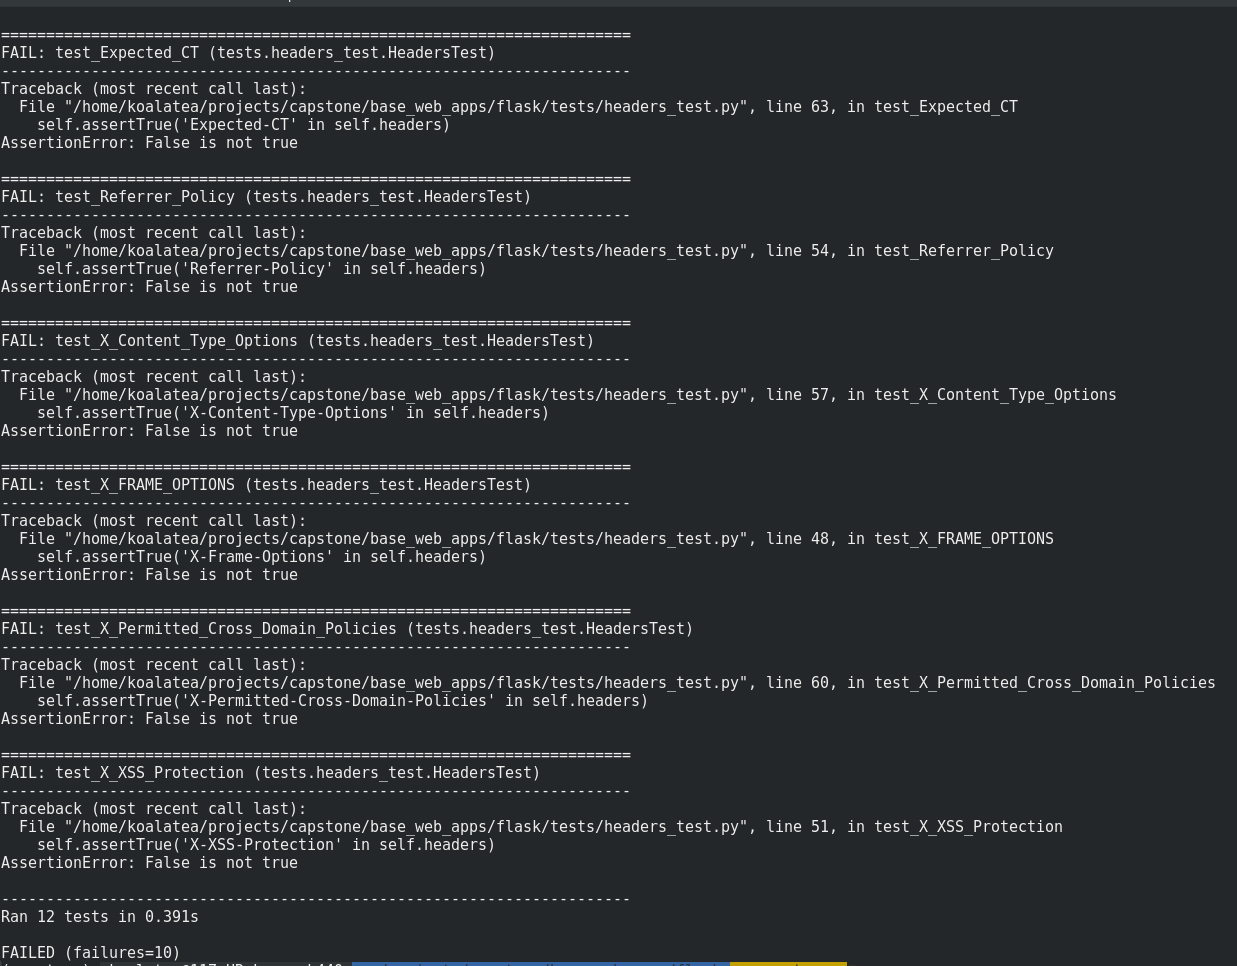
\includegraphics[width=5in]{unittestfail}
\caption{\label{fig:fig2}}Example execution of failing tests
\end{figure}
\begin{figure}[!ht]
  \centering
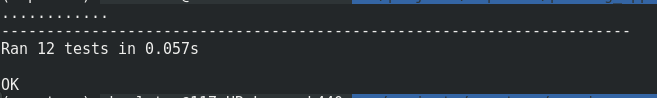
\includegraphics[width=4in]{unittestpass}
\caption{\label{fig:fig3}}Example execution of passing tests
\end{figure}

The HTTPS test is tested by verifying that browsing to HTTP root redirects to an HTTPS root and then that doing a GET request against the HTTPS root returns a 200 response. Following the HTTPS test,
HSTS is tested next by checking the Strict-Transport-Security header and that at least max-age is set, further parts could be included if the developer also wanted includeSubDomains or preload. CSP
is tested in a similiar way by checking that the Content-Security-Policy header is present and does not have unsafe-inline within any of the Content-Security-Policy headers. The rest of the headers
are implemented soley by checking for their existence. The headers have settings that are too different between projects so they are not tested for. The CSRF test is implemented using a list of
dictionaries to keep track of end points. Each dictionary is of an endpoint that has a form to fill. The dictionaries have the endpoint, data to post, fail$\textunderscore$text which is the text
present if the form submission failed, success$\textunderscore$text which is the text present if the form submission succeeds, a fail$\textunderscore$status$\textunderscore$code which is the status
code for a failed submission, and a success$\textunderscore$status$\textunderscore$code if the submission succeeds. In the case of there not being one of the four success or fail codes or text then
they are set to none. In the CSRF test for each endpoint the endpoint is queried and is searched for an input html tag with an id of csrf$\textunderscore$token. If the csrf$\textunderscore$token
exists the endpoint is POSTed to without the token. The response to this post is checked for each fail condition that is not none, and reach success condition that is not none is checked to make sure
they are absent. Finally the csrf$\textunderscore$token found earlier is added to the data and POSTed again with the checks from the POST without the token are reversed. The rest of the tests are
static tests. Only one was implemented because it was found that the rest of the planned ones were already implemented. The os tests are done for potential inject points using os, which is slightly
different from the original goal in the checks list, but the crypto one does exactly what is being looked for by checking for depreciated crypto. The written test was written as a plugin for bandit,
it checks for any print statements and recommends using a logging library instead. This one exists partially because most developers already use logging libraries for most projects, the other reason
is for propper logging management to avoid resource exhaustion.

All of the dynamic tests were easy to transfer over to java, only the url and the requests library had to be changed and the test functioned that same. The caveat is that the java application had to
be dockerized so that it could be tested with the python code, while the python tests worked by using flasks built in debug client. The static tests are not as easy to transfer over. To use the
static test the already implemented tests either needed to be found in another static code analysis tool or writen again for java.

These tests were then added to a CI pipeline in Travis. To do so build stages were used for parallelizing the tests. In this project this made sense because there were two passing and two failing
builds. Figure~\ref{fig:fig4} is the travis.yml configuration file.
\begin{figure}[!ht]
  \centering
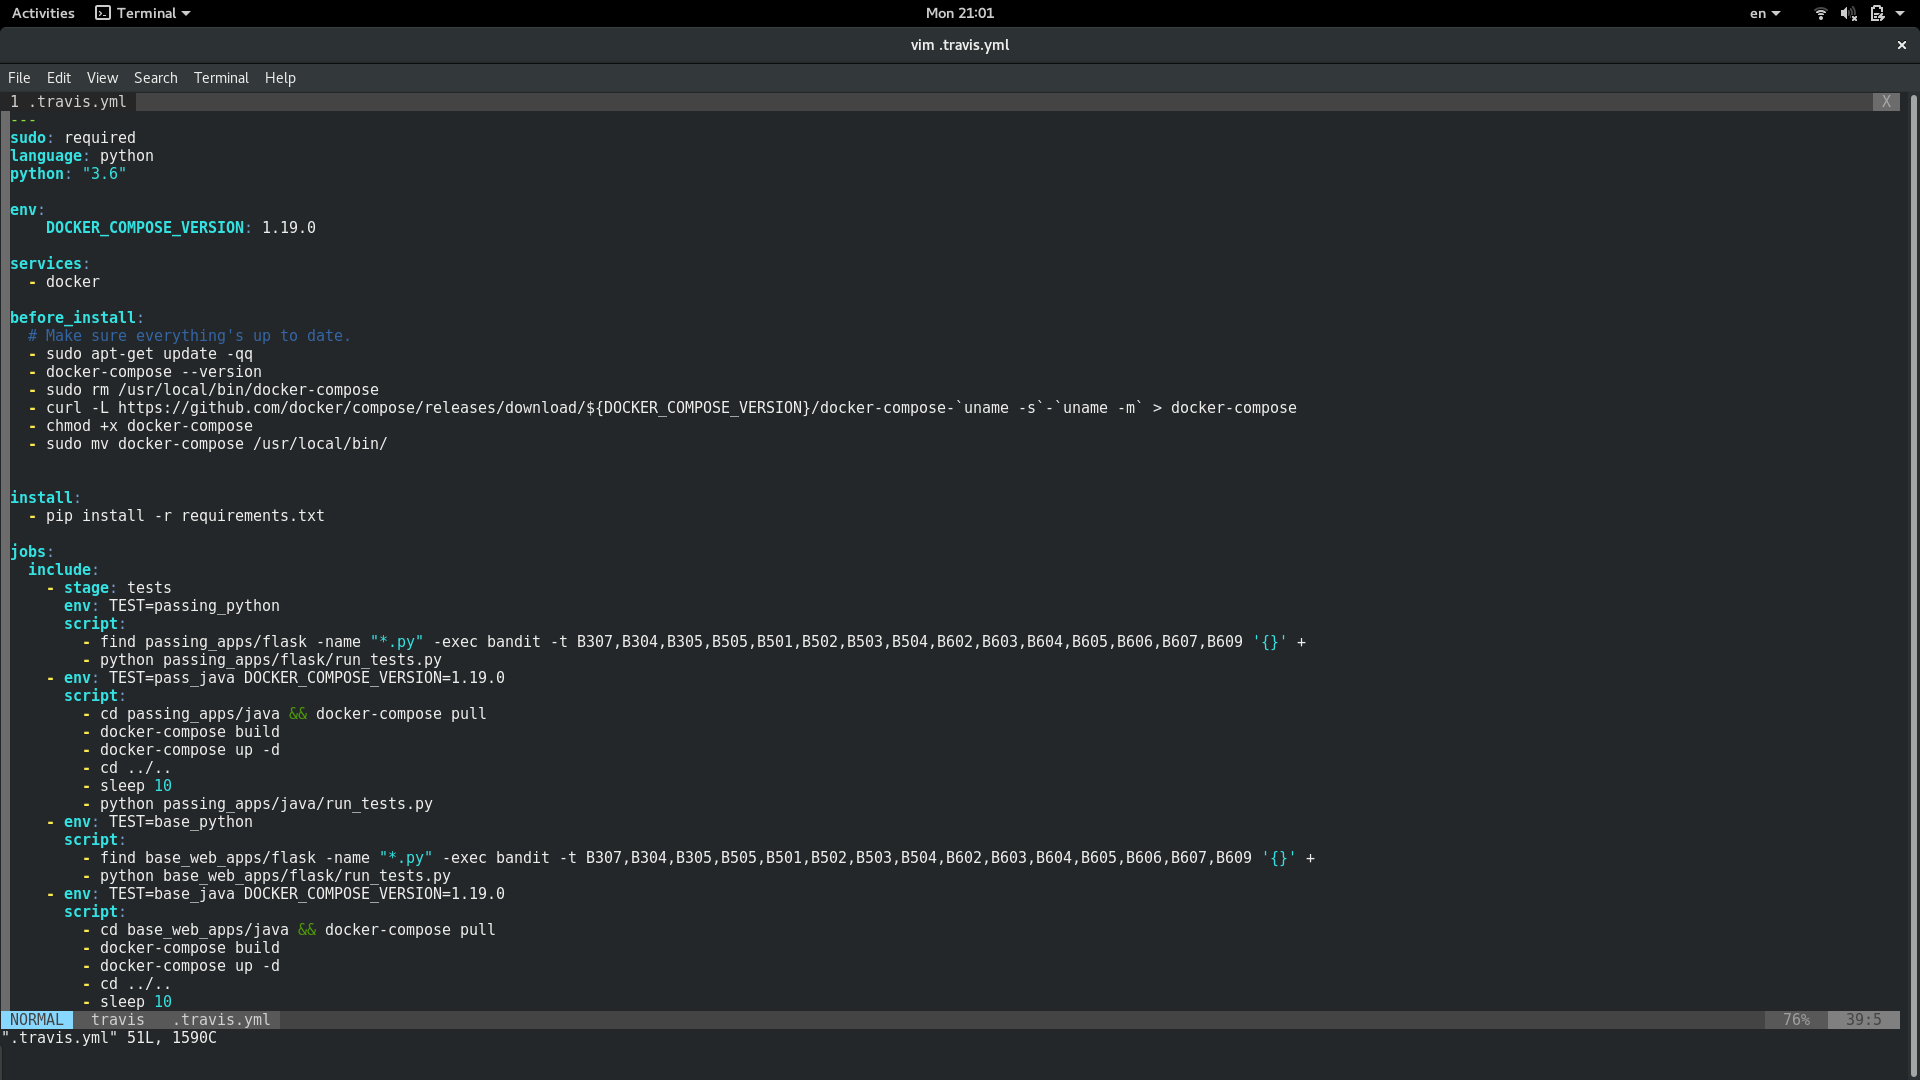
\includegraphics[width=6in]{travis}
\caption{\label{fig:fig4}}The travis configuration file
\end{figure}
The configuration involved install steps that installed docker-compose. This is required for running the dynamic tests against java, since it cannot just hook into the internal testing tools like
with flask. There are also settings for what version of python this project uses, that sudo is required, and docker needs to be installed. Then the stages are defined. There are two stages for python
and two for java. The TEST environment variables are set for visability into what each build is doing from the travis webpage. In both python builds, first bandit is run against it with the tests
that address the use of subproccess, os, and crypto. Next the unit tests are run against the flask. For the java, first docker is set up and then the unit tests are run against them. If any of the
static tests trigger or the unittests fail, then the entire build will fail. Figure~\ref{fig:fig5} shows an example of the builds being ran in travis.
\begin{figure}[!ht]
  \centering
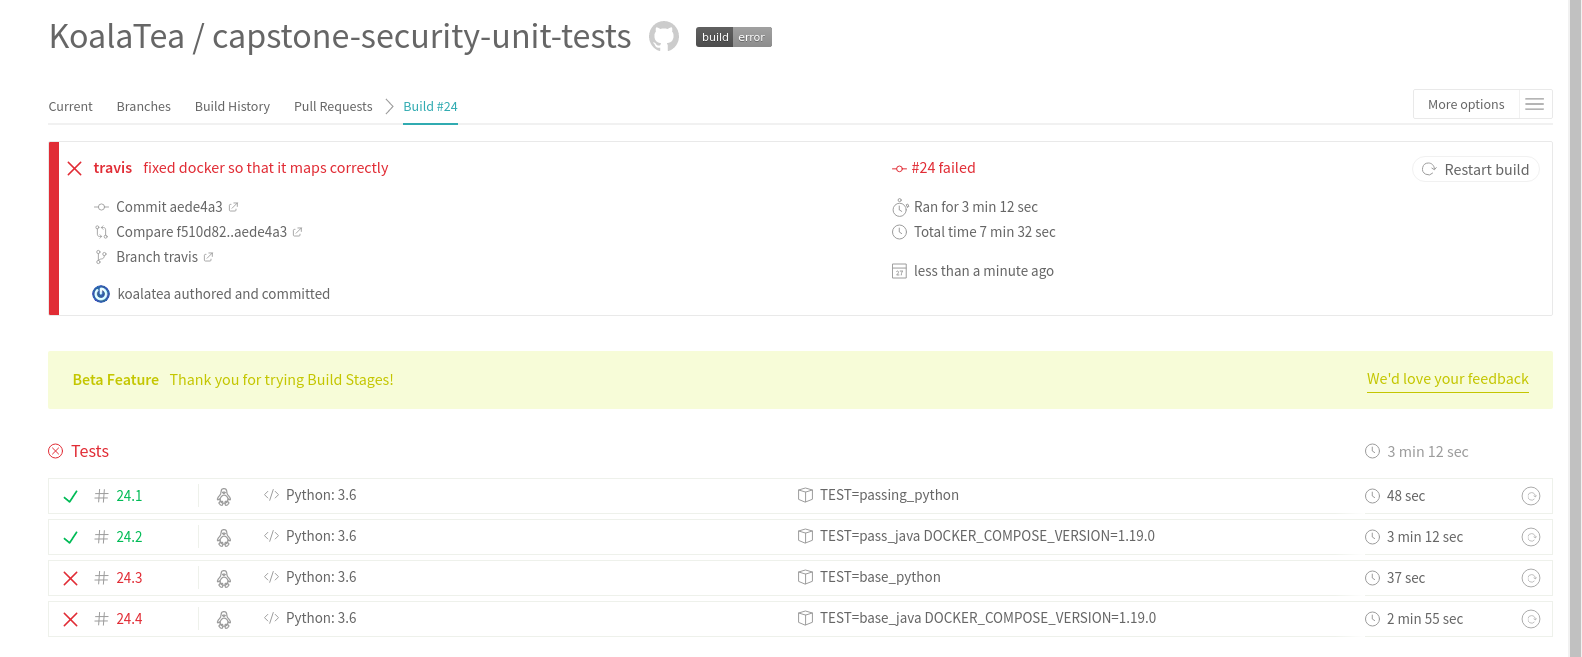
\includegraphics[width=6in]{travisbuilds}
\caption{\label{fig:fig5}}Builds being ran in travis
\end{figure}

